%**************************************************************
\subsubsection{Package it.tecsen.smacs}
\label{subsubsec:it-tecsen-smacs}

\begin{figure}[!h] 
  \centering 
  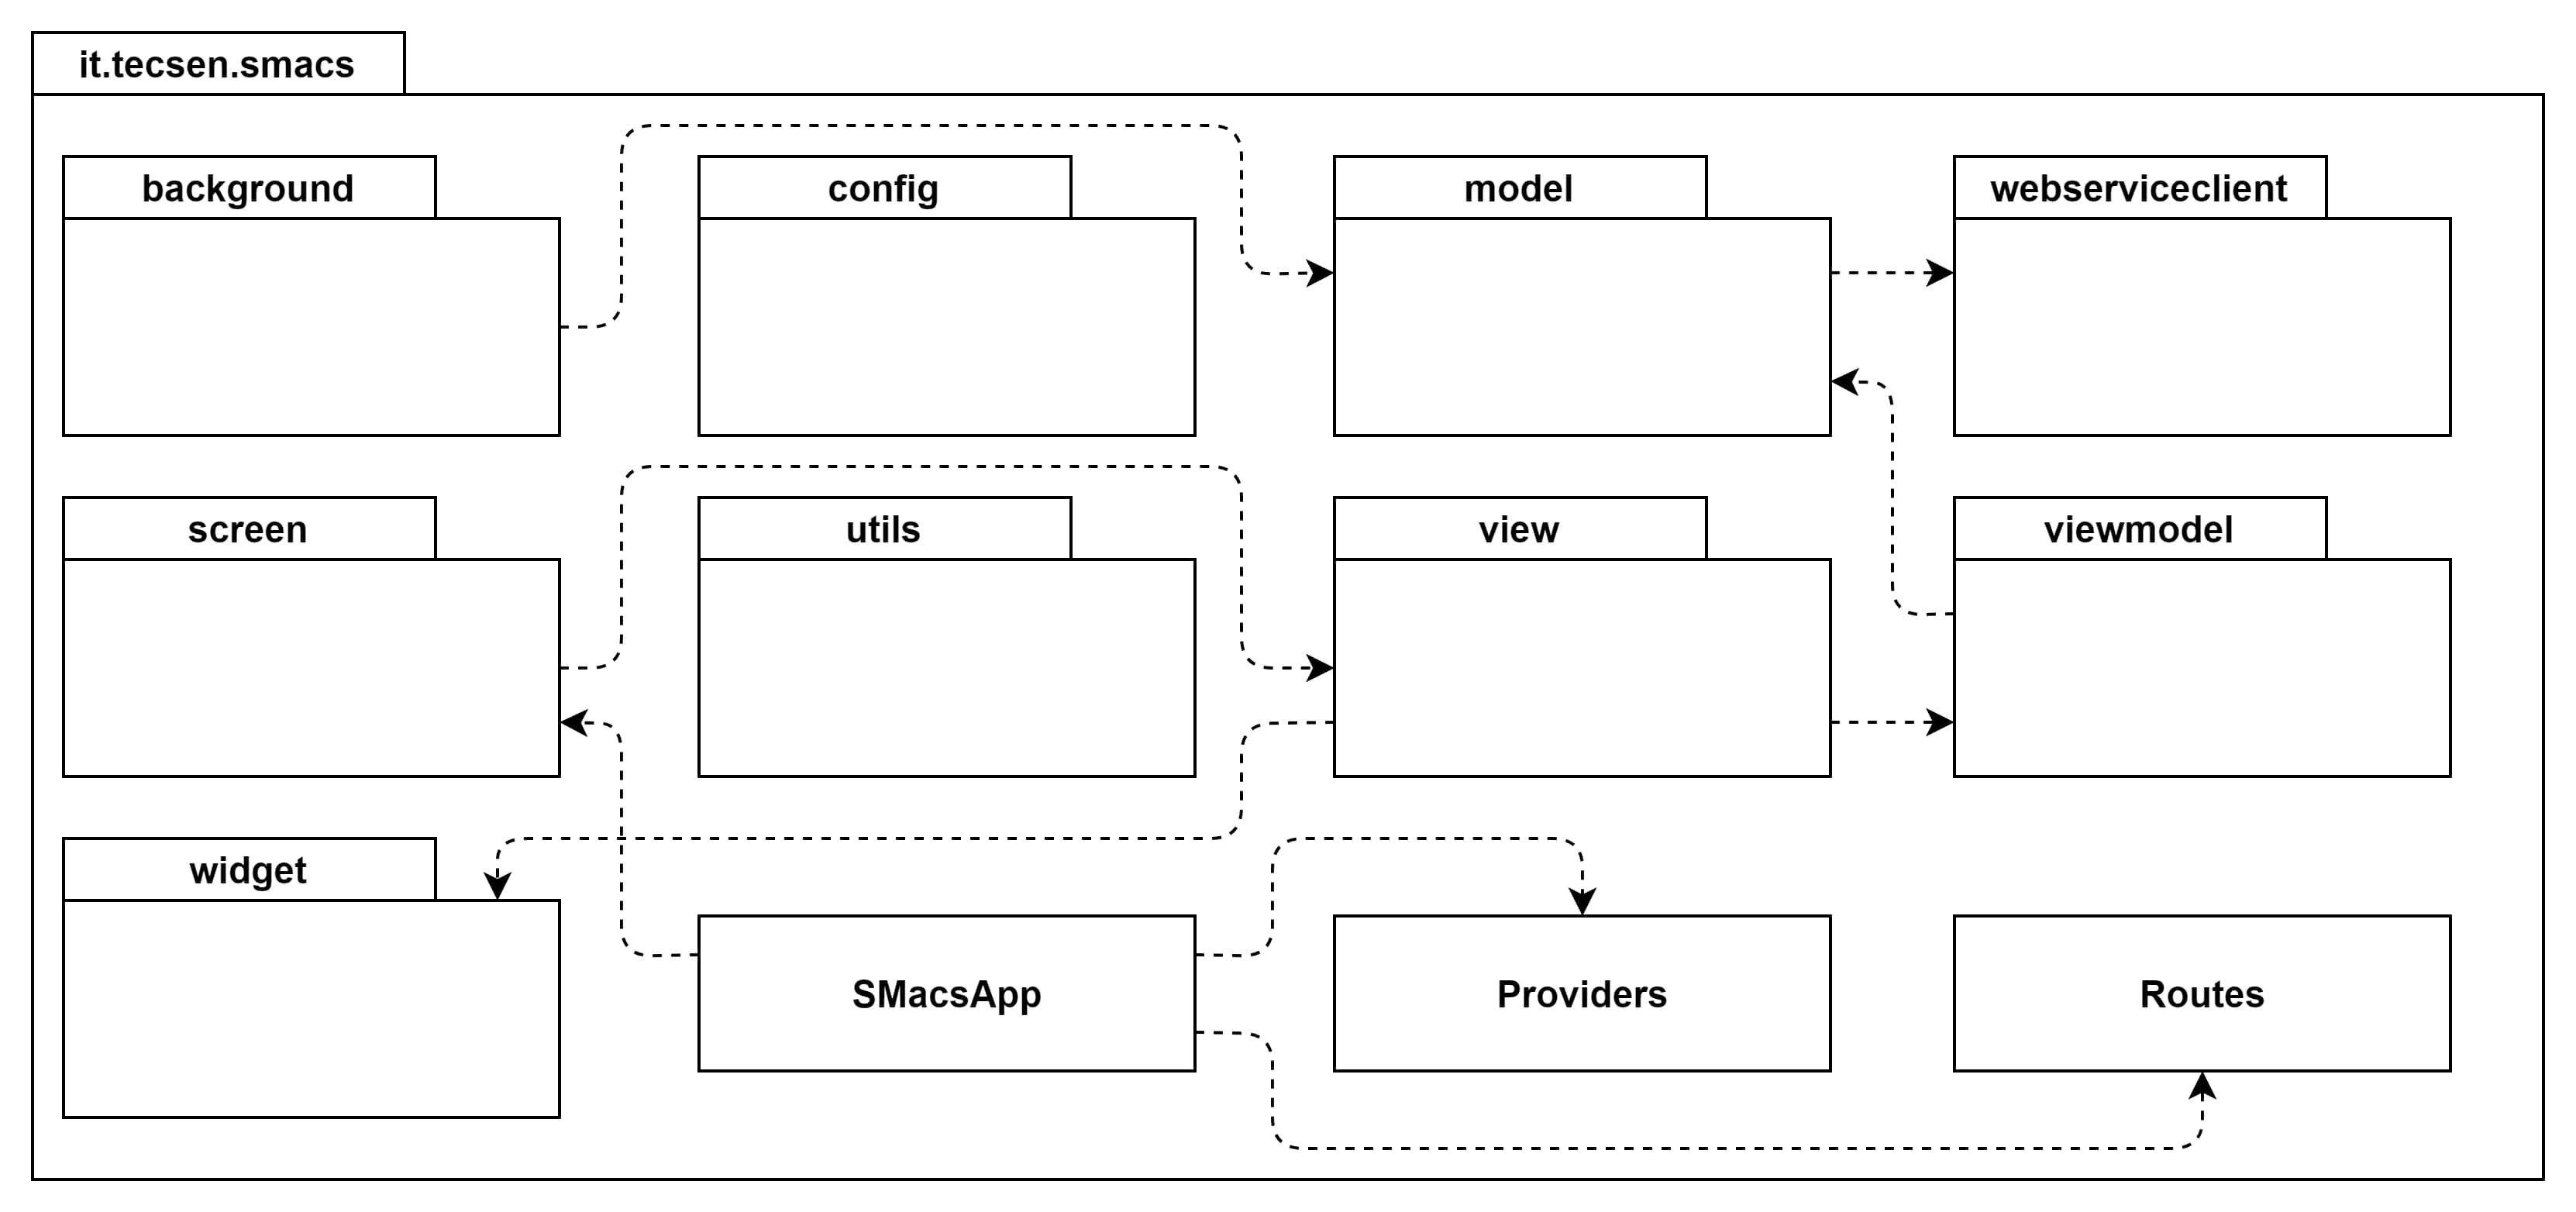
\includegraphics[width=1.0\columnwidth]{capitolo-6/organizzazione-package/it-tecsen-smacs} 
  \caption{Diagramma del package \texttt{it.tecsen.smacs}}
\end{figure}
Il seguente package racchiude tutto il codice sorgente dell'applicazione (non è stato richiesto l'uso del \emph{Platform Channel}), librerie escluse.\\
È suddiviso in più sotto-package seguendo il pattern architetturale Model View ViewModel, per cui sono presenti (come si può vedere nel diagramma sottostante) i package \texttt{model}, \texttt{viewmodel} e \texttt{view}.\\
\textbf{N.B.} Le dipendenze evidenziate nel diagramma sono quelle principali. Ad esempio, quasi tutti i package dipendono da \texttt{utils} e \texttt{config}, dato che contengono rispettivamente classi di utilità e di configurazione, ma non sono state segnate.\\
I package \texttt{screen} e \texttt{widget} fanno sempre parte del concetto \texttt{view} del pattern, ma sono separate dal package \emph{view} per ragioni organizzative:
\begin{itemize}
  \item \texttt{screen} contiene le classi che implementano i widget radice di ogni schermata dell'applicazione. Ognuno di questi widget è ridotto al minimo essenziale per poter poi utilizzare un widget dichiarato nel package \texttt{view} come resto del \emph{Widget tree};
  \item \texttt{widget} contiene le classi che implementano alcuni widget usati dalle classi in \texttt{screen} e \texttt{view}, a scopo di riutilizzo.
\end{itemize}
I package \texttt{model}, \texttt{viewmodel} e \texttt{view} contengono le classi per svolgere il loro ruolo all'interno dell'architettura.\\
Il package \texttt{utils} contiene classi con metodi di utilità (per esempio per il parsing di UUID, per l'hashing di stringhe, per la gestione di date, del logging e altro).\\
Il package \texttt{config} contiene classi con la configurazione dell'app, di alcuni plugin (come quello per la pubblicazione di notifiche), dell'internazionalizzazione e mappe per analizzare i dati ricevuti dalle \gls{restg}.\\
Il package \texttt{webserviceclient} contiene l'implementazione di un semplice wrapper di alcuni metodi della libreria \emph{http}\footcite{site:http-library} per facilitarne l'uso all'interno delle classi del package \texttt{model}.\\
Infine, \texttt{SMacsApp} è la classe che implementa il widget radice dell'intera applicazione e si serve delle classi \texttt{Routes} e \texttt{Providers} in cui sono presenti rispettivamente la configurazione della navigazione all'interno dell'app e le dipendenze di tutte le classi del package \texttt{viewmodel}.
